\subsubsection {Étape 3 : Démarrez Cassandra à partir de Windows CMD:}
Accédez au dossier Cassandra bin. Démarrez l'invite de commande Windows directement à partir du dossier bin en tapant cmd dans la barre d'adresse et en appuyant sur Entrée .

\begin{figure}[h]
	\centering
    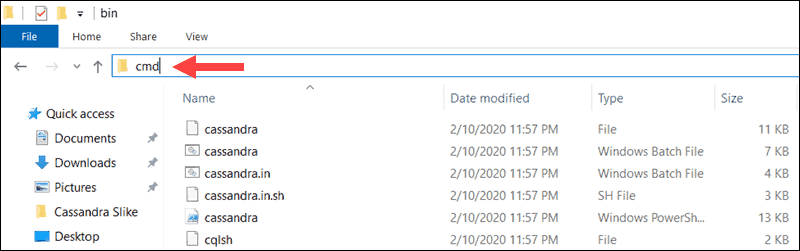
\includegraphics[scale=0.6]{img/part3/2.5}
    \caption{dossier Cassandra bin}
\end{figure}

Tapez la commande suivante pour démarrer le serveur Cassandra :

\begin{center}
$cassandra$
\end{center}

Le système démarre le serveur Cassandra.

\begin{figure}[h]
	\centering
    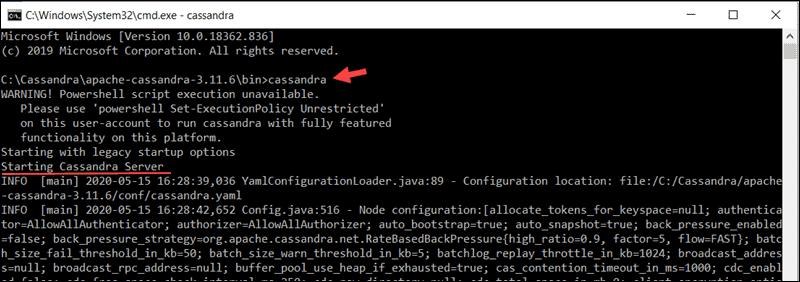
\includegraphics[scale=0.6]{img/part3/2.6}
    \caption{le serveur Cassandra}
\end{figure}

Ne fermez pas la session cmd en cours.